\documentclass{standalone}
\usepackage{tikz}
\usetikzlibrary{patterns, positioning}


\begin{document}
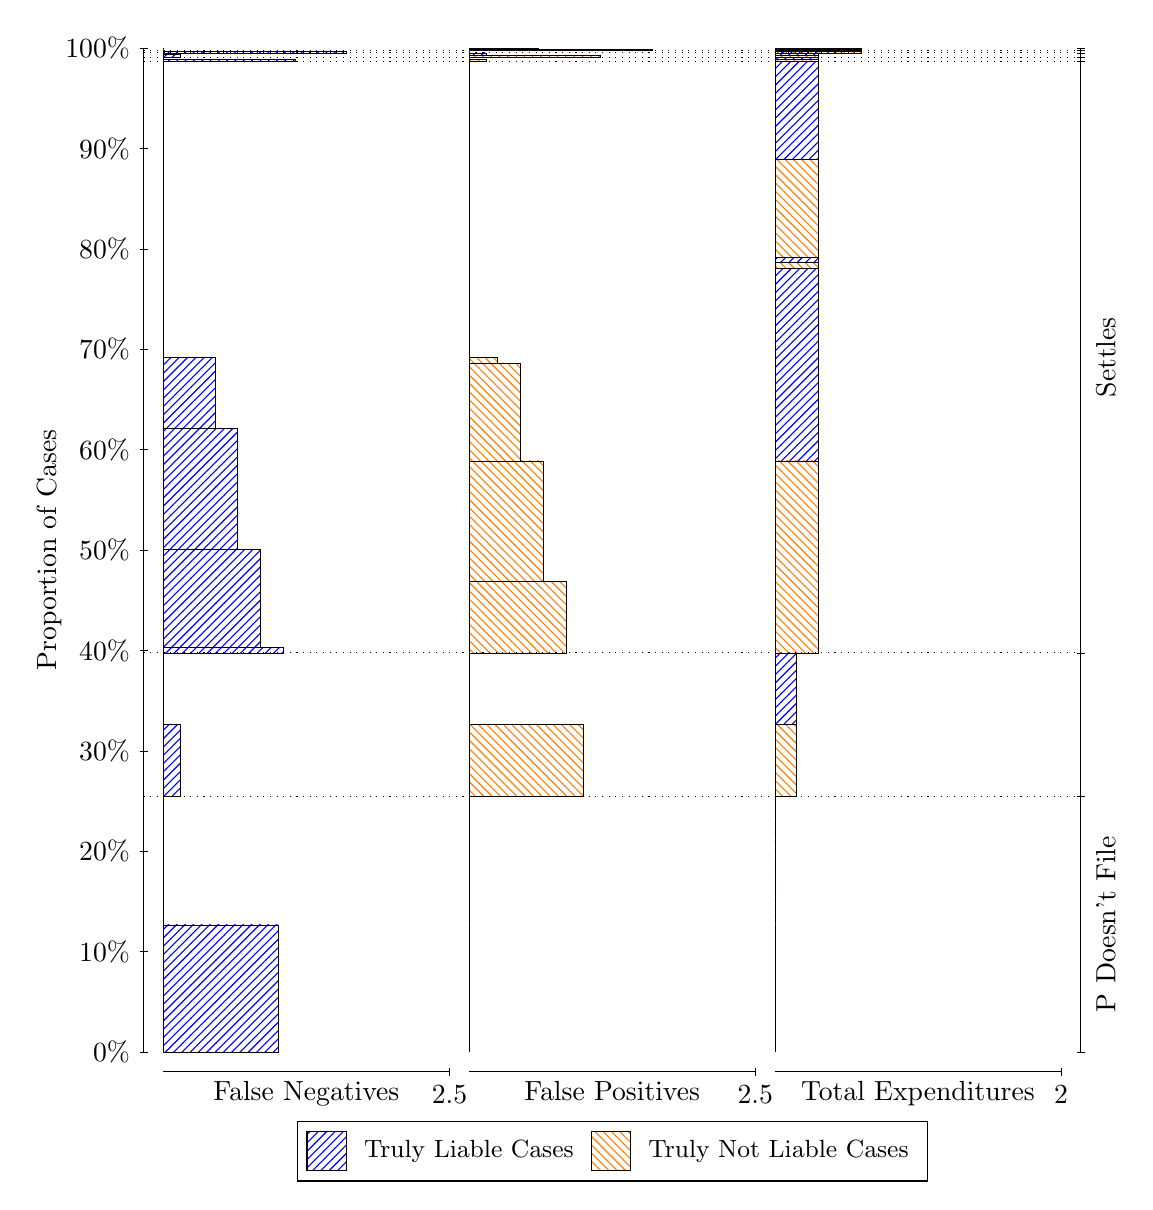
\begin{tikzpicture}
\draw[black, very thin] (1.5,1.75) -- (1.5,14.5);
\node[rotate=90, text=black, anchor=center] at (0.3, 8.125) {Proportion of Cases};
\draw[black, very thin] (1.45,1.75) -- (1.55,1.75);
\node[text=black, anchor=east] at (1.45, 1.75) {0\%};
\draw[black, very thin] (1.45,3.025) -- (1.55,3.025);
\node[text=black, anchor=east] at (1.45, 3.025) {10\%};
\draw[black, very thin] (1.45,4.3) -- (1.55,4.3);
\node[text=black, anchor=east] at (1.45, 4.3) {20\%};
\draw[black, very thin] (1.45,5.575) -- (1.55,5.575);
\node[text=black, anchor=east] at (1.45, 5.575) {30\%};
\draw[black, very thin] (1.45,6.85) -- (1.55,6.85);
\node[text=black, anchor=east] at (1.45, 6.85) {40\%};
\draw[black, very thin] (1.45,8.125) -- (1.55,8.125);
\node[text=black, anchor=east] at (1.45, 8.125) {50\%};
\draw[black, very thin] (1.45,9.4) -- (1.55,9.4);
\node[text=black, anchor=east] at (1.45, 9.4) {60\%};
\draw[black, very thin] (1.45,10.675) -- (1.55,10.675);
\node[text=black, anchor=east] at (1.45, 10.675) {70\%};
\draw[black, very thin] (1.45,11.95) -- (1.55,11.95);
\node[text=black, anchor=east] at (1.45, 11.95) {80\%};
\draw[black, very thin] (1.45,13.225) -- (1.55,13.225);
\node[text=black, anchor=east] at (1.45, 13.225) {90\%};
\draw[black, very thin] (1.45,14.5) -- (1.55,14.5);
\node[text=black, anchor=east] at (1.45, 14.5) {100\%};

\draw[black, very thin] (13.4,1.75) -- (13.4,14.5);
\draw[black, very thin] (13.35,1.75) -- (13.45,1.75);
\node[anchor=west] at (13.35, 1.75) {};
\draw[black, very thin] (13.35,4.9973) -- (13.45,4.9973);
\node[anchor=west] at (13.35, 4.9973) {};
\draw[black, very thin] (13.35,6.8187) -- (13.45,6.8187);
\node[anchor=west] at (13.35, 6.8187) {};
\draw[black, very thin] (13.35,14.328) -- (13.45,14.328);
\node[anchor=west] at (13.35, 14.328) {};
\draw[black, very thin] (13.35,14.378) -- (13.45,14.378);
\node[anchor=west] at (13.35, 14.378) {};
\draw[black, very thin] (13.35,14.439) -- (13.45,14.439);
\node[anchor=west] at (13.35, 14.439) {};
\draw[black, very thin] (13.35,14.469) -- (13.45,14.469);
\node[anchor=west] at (13.35, 14.469) {};
\draw[black, very thin] (13.35,14.5) -- (13.45,14.5);
\node[anchor=west] at (13.35, 14.5) {};

\draw[black, very thin, pattern color=blue, pattern=north east lines] (1.75,1.75) rectangle (3.2033,3.3628);
\draw[black, very thin, pattern color=orange, pattern=north west lines] (1.75,3.3628) rectangle (1.75,4.9973);
\draw[black, very thin, pattern color=blue, pattern=north east lines] (1.75,4.9973) rectangle (1.968,5.908);
\draw[black, very thin, pattern color=orange, pattern=north west lines] (1.75,5.908) rectangle (1.75,6.8187);
\draw[black, very thin, pattern color=blue, pattern=north east lines] (1.75,6.8187) rectangle (3.276,6.8866);
\draw[black, very thin, pattern color=blue, pattern=north east lines] (1.75,6.8866) rectangle (2.9853,8.1335);
\draw[black, very thin, pattern color=blue, pattern=north east lines] (1.75,8.1335) rectangle (2.6947,9.6654);
\draw[black, very thin, pattern color=blue, pattern=north east lines] (1.75,9.6654) rectangle (2.404,10.576);
\draw[black, very thin, pattern color=orange, pattern=north west lines] (1.75,10.576) rectangle (1.75,14.328);
\draw[black, very thin, pattern color=blue, pattern=north east lines] (1.75,14.328) rectangle (3.4213,14.353);
\draw[black, very thin, pattern color=orange, pattern=north west lines] (1.75,14.353) rectangle (1.75,14.378);
\draw[black, very thin, pattern color=blue, pattern=north east lines] (1.75,14.378) rectangle (1.968,14.415);
\draw[black, very thin, pattern color=orange, pattern=north west lines] (1.75,14.415) rectangle (1.75,14.439);
\draw[black, very thin, pattern color=blue, pattern=north east lines] (1.75,14.439) rectangle (4.0753,14.454);
\draw[black, very thin, pattern color=orange, pattern=north west lines] (1.75,14.454) rectangle (1.75,14.469);
\draw[black, very thin, pattern color=orange, pattern=north west lines] (1.75,14.469) rectangle (1.75,14.483);
\draw[black, very thin, pattern color=blue, pattern=north east lines] (1.75,14.483) rectangle (1.75,14.5);
\draw[black, very thin, pattern color=orange, pattern=north west lines] (5.6333,1.75) rectangle (5.6333,3.3845);
\draw[black, very thin, pattern color=blue, pattern=north east lines] (5.6333,3.3845) rectangle (5.6333,4.9973);
\draw[black, very thin, pattern color=orange, pattern=north west lines] (5.6333,4.9973) rectangle (7.0867,5.908);
\draw[black, very thin, pattern color=blue, pattern=north east lines] (5.6333,5.908) rectangle (5.6333,6.8187);
\draw[black, very thin, pattern color=orange, pattern=north west lines] (5.6333,6.8187) rectangle (6.8687,7.7294);
\draw[black, very thin, pattern color=orange, pattern=north west lines] (5.6333,7.7294) rectangle (6.578,9.2572);
\draw[black, very thin, pattern color=orange, pattern=north west lines] (5.6333,9.2572) rectangle (6.2873,10.497);
\draw[black, very thin, pattern color=orange, pattern=north west lines] (5.6333,10.497) rectangle (5.9967,10.571);
\draw[black, very thin, pattern color=blue, pattern=north east lines] (5.6333,10.571) rectangle (5.6333,14.328);
\draw[black, very thin, pattern color=orange, pattern=north west lines] (5.6333,14.328) rectangle (5.8513,14.353);
\draw[black, very thin, pattern color=blue, pattern=north east lines] (5.6333,14.353) rectangle (5.6333,14.378);
\draw[black, very thin, pattern color=orange, pattern=north west lines] (5.6333,14.378) rectangle (7.3047,14.403);
\draw[black, very thin, pattern color=blue, pattern=north east lines] (5.6333,14.403) rectangle (5.8513,14.439);
\draw[black, very thin, pattern color=orange, pattern=north west lines] (5.6333,14.439) rectangle (5.6333,14.455);
\draw[black, very thin, pattern color=blue, pattern=north east lines] (5.6333,14.455) rectangle (5.6333,14.469);
\draw[black, very thin, pattern color=orange, pattern=north west lines] (5.6333,14.469) rectangle (7.9587,14.483);
\draw[black, very thin, pattern color=blue, pattern=north east lines] (5.6333,14.483) rectangle (6.5053,14.5);
\draw[black, very thin, pattern color=orange, pattern=north west lines] (9.5167,1.75) rectangle (9.5167,3.3845);
\draw[black, very thin, pattern color=blue, pattern=north east lines] (9.5167,3.3845) rectangle (9.5167,4.9973);
\draw[black, very thin, pattern color=orange, pattern=north west lines] (9.5167,4.9973) rectangle (9.7892,5.908);
\draw[black, very thin, pattern color=blue, pattern=north east lines] (9.5167,5.908) rectangle (9.7892,6.8187);
\draw[black, very thin, pattern color=orange, pattern=north west lines] (9.5167,6.8187) rectangle (10.062,9.2572);
\draw[black, very thin, pattern color=blue, pattern=north east lines] (9.5167,9.2572) rectangle (10.062,11.7);
\draw[black, very thin, pattern color=orange, pattern=north west lines] (9.5167,11.7) rectangle (10.062,11.773);
\draw[black, very thin, pattern color=blue, pattern=north east lines] (9.5167,11.773) rectangle (10.062,11.841);
\draw[black, very thin, pattern color=orange, pattern=north west lines] (9.5167,11.841) rectangle (10.062,13.081);
\draw[black, very thin, pattern color=blue, pattern=north east lines] (9.5167,13.081) rectangle (10.062,14.328);
\draw[black, very thin, pattern color=orange, pattern=north west lines] (9.5167,14.328) rectangle (10.062,14.353);
\draw[black, very thin, pattern color=blue, pattern=north east lines] (9.5167,14.353) rectangle (10.062,14.378);
\draw[black, very thin, pattern color=orange, pattern=north west lines] (9.5167,14.378) rectangle (10.062,14.403);
\draw[black, very thin, pattern color=blue, pattern=north east lines] (9.5167,14.403) rectangle (10.062,14.439);
\draw[black, very thin, pattern color=orange, pattern=north west lines] (9.5167,14.439) rectangle (10.607,14.455);
\draw[black, very thin, pattern color=blue, pattern=north east lines] (9.5167,14.455) rectangle (10.607,14.469);
\draw[black, very thin, pattern color=orange, pattern=north west lines] (9.5167,14.469) rectangle (10.607,14.483);
\draw[black, very thin, pattern color=blue, pattern=north east lines] (9.5167,14.483) rectangle (10.607,14.5);
\draw[black, dotted] (1.5,4.9973) -- (13.4,4.9973);
\draw[black, dotted] (1.5,6.8187) -- (13.4,6.8187);
\draw[black, dotted] (1.5,14.328) -- (13.4,14.328);
\draw[black, dotted] (1.5,14.378) -- (13.4,14.378);
\draw[black, dotted] (1.5,14.439) -- (13.4,14.439);
\draw[black, dotted] (1.5,14.469) -- (13.4,14.469);
\draw[black, very thin] (1.75,1.5) -- (5.3833,1.5);
\node[text=black, anchor=north] at (3.5667, 1.5) {False Negatives};
\draw[black, very thin] (5.3833,1.45) -- (5.3833,1.55);
\node[text=black, anchor=north] at (5.3833, 1.45) {2.5};

\draw[black, very thin] (5.6333,1.5) -- (9.2667,1.5);
\node[text=black, anchor=north] at (7.45, 1.5) {False Positives};
\draw[black, very thin] (9.2667,1.45) -- (9.2667,1.55);
\node[text=black, anchor=north] at (9.2667, 1.45) {2.5};

\draw[black, very thin] (9.5167,1.5) -- (13.15,1.5);
\node[text=black, anchor=north] at (11.333, 1.5) {Total Expenditures};
\draw[black, very thin] (13.15,1.45) -- (13.15,1.55);
\node[text=black, anchor=north] at (13.15, 1.45) {2};

\node[text=black, centered, rotate=90] at (13.72, 3.3736) {P Doesn't File};

\node[text=black, centered, rotate=90] at (13.72, 10.573) {Settles};





\draw (7.449999999999999,1.5) node[draw=none] (baseCoordinate) {};
\begin{scope}[align=center]
        \matrix[scale=0.5, draw=black, below=0.5cm of baseCoordinate, nodes={draw}, column sep=0.1cm]{
            \node[rectangle, draw, minimum width=0.5cm, minimum height=0.5cm, pattern color=blue, pattern=north east lines] {}; &
            \node[draw=none, font=\small, text=black] (B) {Truly Liable Cases}; &
            \node[rectangle, draw, minimum width=0.5cm, minimum height=0.5cm, pattern color=orange, pattern=north west lines] {}; &
            \node[draw=none, font=\small, text=black] (B) {Truly Not Liable Cases}; \\
            };
\end{scope}

\end{tikzpicture}
\end{document}